\documentclass{article}
\usepackage{amssymb}
\usepackage{amsmath}
\usepackage{hyperref}
\usepackage{graphicx}
\setlength{\parindent}{0pt}
\begin{document}

\title{IVR Assignment}
\author{Joseph Abboud and Marley Adair}
\date{}
\maketitle

Joseph Abboud worked on implementing the robot control section. Marley Adair worked on implementing the robot vision section. The project is available on github at \url{https://github.com/gemdude46/ivr_assignment}. \\

\section{Robot Vision}

\subsection{Joint state estimation}

In order to determine the joint states, the program takes the coloured sections for each joint colour from both viewpoints, and uses their moments to determine where they are centred from both perspectives. Then, a ray is cast from each camera out from the centre, and
the closest approach between the lines is used as the coordinates of that joint. In the event the joint is obscured from the perspective of one camera, the rays of all other objects the joint could be obscured behind are tested, and the one with the closest approach
is used. This, however, can still cause errors when the joint is obscured by something that is not a target, such as the connections between joints. \\

After finding the positions of the joints, the angle between the links can be used to find the actual values passed to the robot controller. Figure \ref{fig:visionjointplot} shows the outputs of this algorithm compared to the actual values sent to the joints. Note that
the estimates may be shifted in time due to the latency of processing the images. \\

\begin{figure}
	\makebox[\textwidth][c]{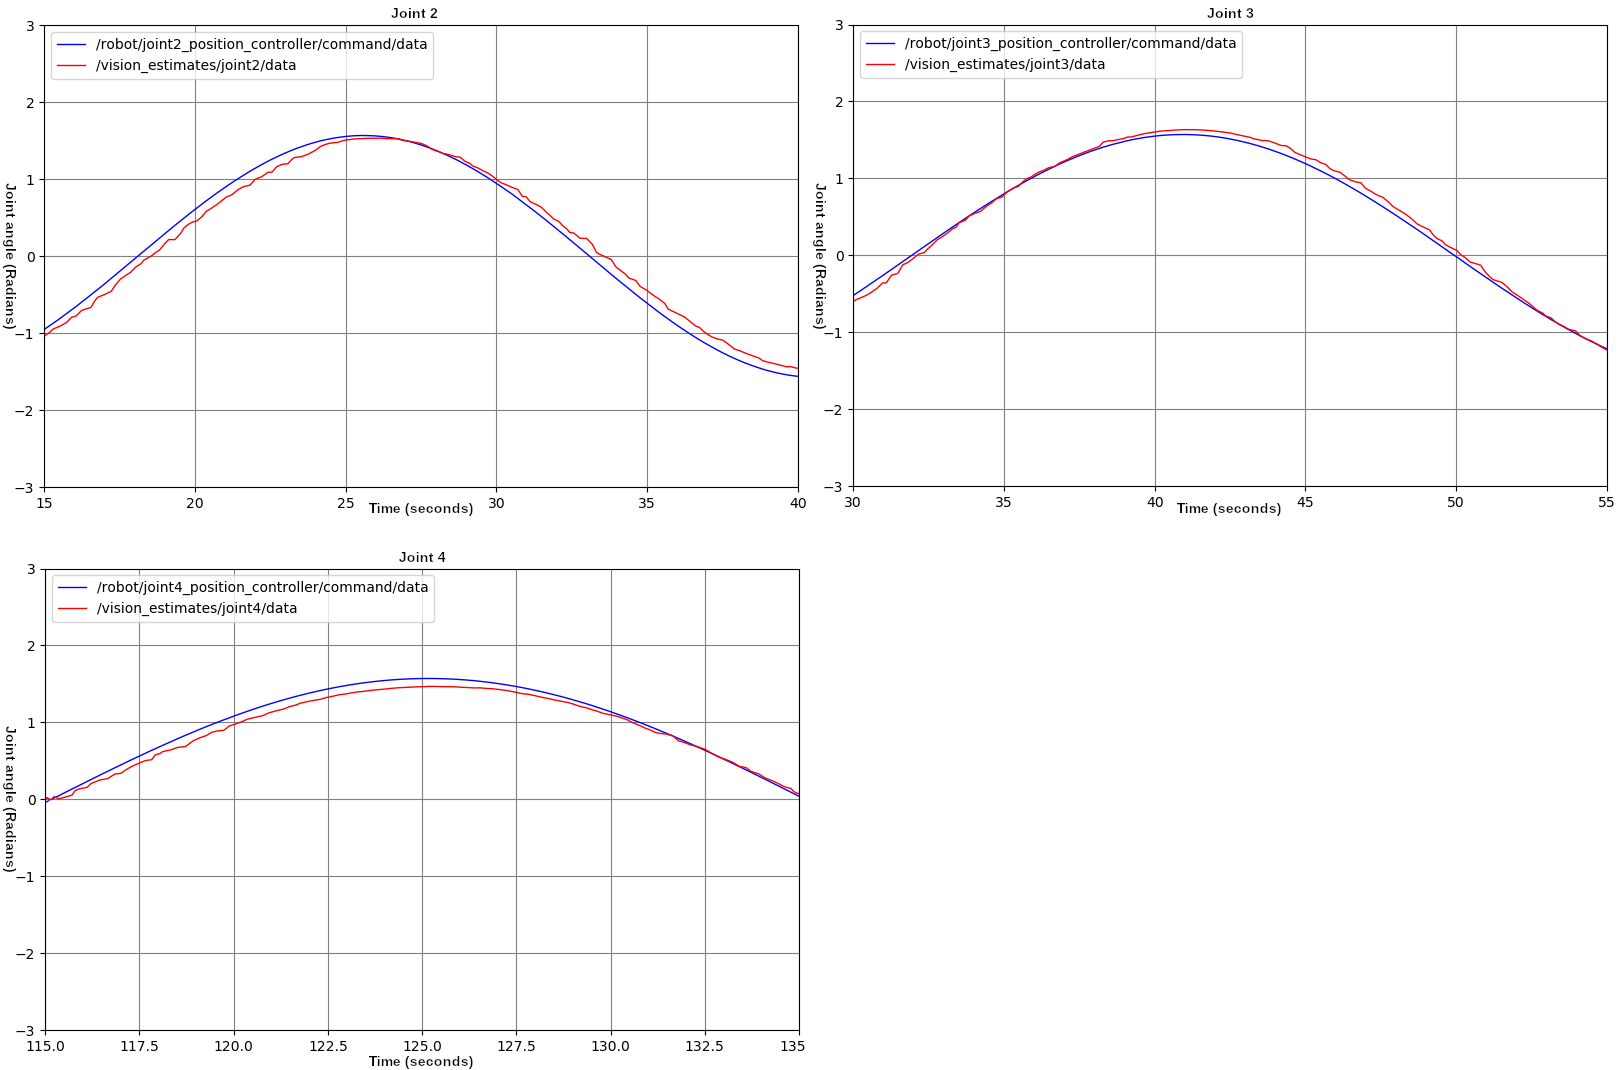
\includegraphics[width=19cm]{visionjointplot.png}}
	\caption{Joint values over time.}
	\label{fig:visionjointplot}
\end{figure}

\subsection{Target detection}

In order to seperate the target from the box, the contours of the orange sections are taken. To determine which one is the target, the shape of the bounding box of each contour is used, and the closest to square is the target. While this works the majority of the time,
there are occations, such as when the target is occluded by a link such that it is split into two long thin sections, when this will incorrectly pick the wrong target. Figure \ref{fig:visiontargetplot} shows the actual and calculated positions of the target. \\

\begin{figure}[h]
	\makebox[\textwidth][c]{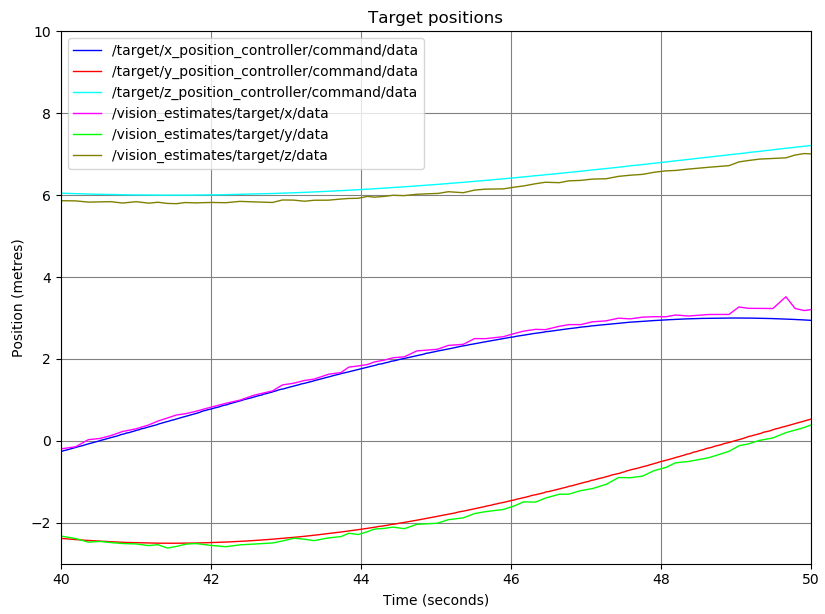
\includegraphics[width=\linewidth]{visiontargetplot.png}}
	\caption{Target position over time.}
	\label{fig:visiontargetplot}
\end{figure}

\section{Robot Control}

Joseph: fill out this section.


\end{document}
